\documentclass{article}
\usepackage{polyglossia}
\usepackage[a4paper,hmargin=4cm]{geometry}
\usepackage{mathtools, amssymb, amsfonts}
\usepackage{amsthm}
\usepackage{fontspec}
\usepackage{titling}
\usepackage{float}
\usepackage{listings}
\usepackage{graphicx}
\usepackage{xcolor}
\usepackage{mdframed}
\usepackage[hidelinks]{hyperref}
\usepackage{caption,subcaption}
\usepackage{tikz}
\usetikzlibrary{arrows,shapes,calc,angles,decorations.markings,patterns,decorations.pathmorphing}
\usepackage[shortlabels]{enumitem}
\usepackage{comment}

\setdefaultlanguage{french}
\frenchspacing

%% Math fonts
\usepackage{unicode-math}
\setmathfont{Latin Modern Math}
%\setmathfont{xits-math.otf}
\setmathfont[range={\mathbb,\mathcal,\mathsf}]{xits-math.otf}
%\setmathfont[range={\mathbb,\mathcal,\mathsf}]{STIXTwoMath.otf}

\newcommand{\NN}{\mathbb N}
\newcommand{\ZZ}{\mathbb Z}
\newcommand{\RR}{\mathbb R}
\newcommand{\QQ}{\mathbb Q}
\newcommand{\CC}{\mathbb C}
\newcommand{\KK}{\mathbb K}
\newcommand{\PP}{\mathbb P}
\DeclareMathOperator{\Card}{\mathrm{Card}}
\DeclarePairedDelimiterX{\zint}[2]{[\![}{]\!]}{#1,#2}
\DeclarePairedDelimiterX{\abs}[1]{\left\lvert}{\right\rvert}{#1}

%% Titling configuration
\pretitle{\begin{center}\hrulefill\\ \LARGE\textsc}
\posttitle{\vspace{-2mm} \\\hrulefill\end{center}\vspace{-0.5em}}

\title{Exercices de Khôlle -- Terminale S}

\preauthor{\begin{center}}
\author{{\normalfont\scshape Lycée Julie-Victoire Daubié}}
\postauthor{\end{center}}

\date{}

%% Sectioning


\renewcommand{\thesection}{\arabic{section}}

\newcounter{Exercice}
\makeatletter
\newcommand{\exercice}[1][\@nil]{\refstepcounter{Exercice}
	\section*{Exercice \theExercice
	\def\tmp{#1}
	\ifx\tmp\@nnil
	%
	\else
	(#1)
	\fi
}}

\makeatother

\begin{document}
	\maketitle

\exercice[Bordeaux 1980]
Pour tout réel $a$, on définit sur $\RR$ la fonction numérique $f_a$ par \[f_a(x) = e^{-x} + ax.\]
Soit $\mathcal C_a$ sa représentation graphique dans le plan équipé d'un repère orthonormé $(O,\vec{\imath},\vec{\jmath})$.

\begin{enumerate}
	\item Étudier les variations de $f_a$. Pour quelles valeurs de $a$ la fonction $f_a$ admet-elle un extremum ? On appelle $A$ l'ensemble de ces valeurs.
	\item Pour tout tel réel $a\in A$, on appelle $M_a$ le point de $\mathcal C_a$ correspondant à l'extremum. Déterminer ses coordonnées.
	\item Montrer que l'ensemble $E$ des points $M_a$, lorsque $a$ décrit $A$, est la courbe représentative d'une fonction $g$. Étudier les variations de $g$, et dessiner $E$.
\end{enumerate}


\exercice[Paris 1980]

Soit la famille d'équations
\begin{equation}\tag{$E_\theta$}
	z^2\sin^2\theta - 4z\sin\theta + 4 + \cos^2\theta = 0
	\label{eqn:EqTheta}
\end{equation}
où $\theta\in{\left]0,\pi\right[}$.

\begin{enumerate}
	\item Soit $0< \theta< \pi$. Résoudre l'équation \eqref{eqn:EqTheta} dans le corps $\CC$ des nombres complexes. On note $z_1$ et $z_2$ les racines.
	\item On note $M_1$ et $M_2$ dont les nombres complexes $z_1$ et $z_2$ sont les affixes dans un repère orthonormé $(O,\vec u,\vec v)$.\\
	Dessiner l'ensemble des points $M_1$ et $M_2$ lorsque ${]0,\pi[}$.
\end{enumerate}


\exercice[Pondichéry 1996]

Un fabricant de berlingots possède trois machines A, B et C qui fournissent respectivement 10 \%, 40 \% et 50 \% de la production totale de son usine.
Une étude a montré que le pourcentage de berlingots défectueux est de 3,5 \% pour la machine A, de 1,5 \% pour la machine B et de 2,2 \% pour la machine C.
Après fabrication, les berlingots sont versés dans un bac commun aux trois machines.
On choisit au hasard un berlingot dans le bac.

\begin{enumerate}
	\item Montrer que la probabilité que ce berlingot provienne de la machine C et soit défectueux est $0{,}011$.
	\item Calculer la probabilité que ce berlingot soit défectueux.
	\item Calculer la probabilité que ce berlingot provienne de la machine C sachant qu'il est défectueux.
	\item On prélève successivement dans le bac 10 berlingots en remettant à chaque fois le berlingot tiré dans le bac. Calculer la probabilité d'obtenir au moins un berlingot défectueux parmi ces 10 prélèvements.
\end{enumerate}


\exercice[Amérique du Nord 1996]

On désigne par $n$ un entier naturel $\geq 2$. On se donne $n$ sacs de jetons $S_1,\ldots,S_n$. Au départ, le sac $S_1$ contient 2 jetons noirs et 1 jeton blanc, et chacun des autres sacs contient 1 jeton noir et 1 jeton blanc.

On se propose d'étudier l'évolution des tirages successifs d'un jeton de ces sacs, effectuées de la façon suivante:
\begin{itemize}
	\item \textbf{Première étape} on tire au hasard un jeton de $S_1$,
	\item \textbf{Deuxième étape} on place ce jeton de $S_2$ et on tire, au hasard, un jeton de $S_2$,
	\item \textbf{Troisième étape} après avoir placé dans $S_3$ le jeton sorti de $S_2$ on tire, au hasard, un jeton de $S_3$ et ainsi de suite. 
\end{itemize}

\begin{figure}[h]
	\centering
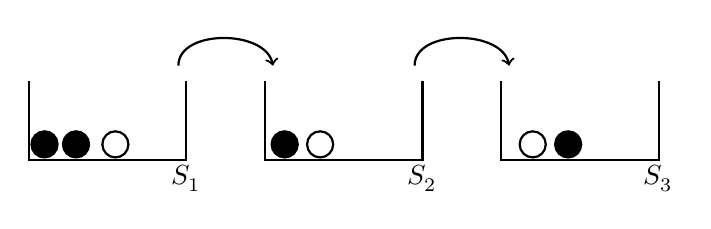
\begin{tikzpicture}
\tikzset{ball/.style={circle, draw=black!100, thick, minimum size=1mm}}
\draw[thick] (-3,1) -- (-3,0) -- (-1,0) -- (-1,1) node[pos=0.2,label=below:$S_1$] {};
\node[ball,fill=black] at (-2.8,0.2) {};
\node[ball,fill=black] at (-2.4,0.2) {};
\node[ball,fill=white] at (-1.9,0.2) {};

\path[thick,out=90,in=100,->] (-1.1,1.2) edge (0.1,1.2);

\draw[thick] (0,1) -- (0,0) -- (2,0) -- (2,1) node[pos=0.2,label=below:$S_2$] {};
\node[ball,fill=black] at (0.25,0.2) {};
\node[ball,fill=white] at (0.7,0.2) {};

\path[thick,out=90,in=100,->] (1.9,1.2) edge (3.1,1.2);

\draw[thick] (3,1) -- (3,0) -- (5,0) -- (5,1) node[pos=0.2,label=below:$S_3$] {};
\node[ball,fill=white] at (3.4,0.2) {};
\node[ball,fill=black] at (3.85,0.2) {};
\end{tikzpicture}
\end{figure}

Pour tout $k\in\NN$ tel que $1\leq k\leq n$, on note $E_k$ l'événement << le jeton sorti de $S_k$ est blanc >> ; on notera classiquement $\overline{E_k}$ son évènement contraire.

\begin{enumerate}
	\item \begin{enumerate}
		\item Déterminer la probabilité de $E_1$ et les probabilités conditionnelles $\PP(E_2|E_1)$ et $\PP(E_2|\overline{E_1})$.\\
		En déduire la probabilité de $E_2$.
		\item Pour tout entier $1\leq k\leq n$, on note la probabilité $\PP(E_k) = p_k$.\\
		Démontrer le relation de récurrence
		\[ p_{k+1} = \frac 1 3 p_k + \frac 1 3. \]
	\end{enumerate}
	\item On définit $(u_k)_{k\geq 1}$ une suite réelle telle que $u_1= \frac 1 3$, telle que 
	\[ u_{k+1} = \frac 1 3 u_k + \frac 1 3.\]
	On pose alors $v_k := u_k - \frac 1 2$.
	\begin{enumerate}
		\item Montrer que la suite $(v_k)$ est géométrique.
		\item En déduire l'expression de $u_k$. Étudier la convergence de la suite $(u_k)$.
	\end{enumerate}
	\item On suppose que $n=10$. Déterminer pour quelles valeurs de $k$ on a
	\[ 0{,}4999\leq p \leq 0{,}5. \]
\end{enumerate}

\exercice[Amiens 1990 (1)]

Soit $f:\CC\rightarrow\CC$ l'application définie par
\[ f(z) = z^4 - \sqrt 2 z^3 - 4\sqrt 2 z - 16. \]

\begin{enumerate}
	\item Calculer $f(2i)$ et $f(-2i)$.
	\item D'après un théorème que l'on admettra, il existe un trinôme du second degré à coefficients réels $q(z)= z^2+az+b$ tel que
	\[ f(z) = (z^2+4)q(z). \]
	Trouver $a$ et $b$.
	\item En déduire les solutions de l'équation $f(z) = 0$ sur $\CC$.
	\item Placer dans le plan complexe rapporté à un repère orthonormé $(O,\vec u,\vec v)$ les points $A,B,C,D$ qui ont pour affixes les solutions de la question précédente.
	\item Montrer que $A,B,C,D$ appartiennent à un même cercle $(\mathcal{C})$ dont on précisera le centre et le rayon.
\end{enumerate}


\exercice[Amiens 1990 (2)]

Pour tout $k > 0$, on considère la fonction $f_k$ définie sur $]0,+\infty[$ par
\[ f_k(x) = k^2x^2 - \frac 1 4 - \frac 1 2 \ln x. \]
On note $\mathcal{C}_k$ sa courbe représentative dans le plan muni d'un repère orthonormé $(O,\vec\imath,\vec{\jmath})$.
\begin{enumerate}
	\item Étudier les variations de $f_k$, dresser son tableau. On précisera les limites de $f_k$.
	\item Soit $M_k$ le point $\mathcal{C}_k$ correspondant au minimum de $f_k$. Déterminer dans le repère $(O,\vec{\imath},\vec{\jmath})$ une équation cartésienne de l'ensemble $\mathcal{A}$ décrit par $M_k$ lorsque $k$ décrit $]0,+\infty[$.
	\item Préciser la position relative de $\mathcal{C}_k$ et $\mathcal{A}$; les tracer. 
\end{enumerate}

\exercice[Amérique du Nord 1986]

Soit, pour tout $z\in\CC$ le polynôme
\[ P_\lambda(z) = z^2 - 4z + \lambda \]
où $\lambda\in\RR$.

\begin{enumerate}
	\item Montrer que si $P_\lambda(z) = 0$ admet une racine $z_\lambda$ alors $\overline{z_\lambda}$ est aussi solution.
	\item Montrer que l'équation $P_\lambda(z) = 0$ admet au moins une solution réelle.
	\item Déterminer $\lambda$ pour que l'équation $P_\lambda(z)=0$ admette au moins une racine réelle de module égal à 2. Résoudre l'équation pour cette valeur de $\lambda$.
	\item Déterminer $\lambda$ pour que $P_\lambda(z)=0$ admette une racine \textbf{complexe} de module égal à 2. Résoudre l'équation pour les valeurs de $\lambda$ trouvées, préciser le module et l'argument de chaque solution.
\end{enumerate}

\exercice[Amérique du Sud 1986]

Soit $P$ le plan complexe muni d'un repère orthonormé $(O,\vec u,\vec v)$. Au points $M(x,y)$ on associe, classiquement, son affixe $z = x+iy$.\\
Soient $A$ et $B$ les points d'affixes respectives $1+i$ et $-3$.

À un point $M$, distinct de $A$ ou $B$ et d'affixe $z$, on associe le(s) point(s) $M'$, s'ils existent, d'affixes $z'$ telles que
\[
\left\{
\begin{array}{ll}
\frac{z'+3}{z+3} &\text{imaginaire pur} \\
\frac{z'-1-i}{z-1-i} &\text{réel}.
\end{array}
\right.
\]

\begin{enumerate}
	\item Donner un sens géométrique à $\arg\left(\dfrac{z'+3}{z+3}\right)$ et $\arg\left(\dfrac{z'-1-i}{z-1-i}\right)$.
	\item Démontrer géométriquement qu'il existe un cercle $\mathcal{C}$ du plan tel que si $M\in P\setminus \mathcal{C}$, alors $M'$ existe et est unique. Construire alors $M'$.
\end{enumerate}


\exercice[Bordeaux 1984]

Soit $\theta\in[0,2\pi]$.
\begin{enumerate}
	\item Résoudre dans $\CC$ l'équation
	\[ z^2 - (2^{\theta+1}\cos\theta)z + 2^{2\theta} = 0, \]
	et donner chaque solution sous forme trigonométrique.
	\item Le plan étant rapporté à un repère orthonormé $(O,\vec u,\vec v)$, on considère les points $A$ et $B$ dont les affixes sont les solutions de l'équation précédente. Déterminer $\theta$ de manière à ce que le triangle $OAB$ soit équilatéral.
\end{enumerate}


\exercice[Montpellier 1984]

On ramène la plan à un repère orthonormé $(O,\vec \imath,\vec \jmath)$. Soit $f$ l'application définie sur $\RR$ par
\[ 
\begin{cases}
f(x) = x \ln\left(1+\frac 1 x\right) &\forall x > 0 \\
f(0) = 0. &
\end{cases}
 \]

\begin{enumerate}
	\item Étudier la continuité et la dérivabilité de $f$ en $0$.
	\item On considère la fonction $g$ définie sur $[1,+\infty[$ par
	\[ g(x) = x\ln x \]
	et on appelle $\Gamma$ sa courbe représentative. Étudier $g$ et tracer $\Gamma$.
	\item Étudier la limite $f$ en $+\infty$. Montrer que les courbes $\Gamma$ et $\mathcal{C}$ sont asymptotes l'une de l'autre et préciser leur positions relatives.\\
	\textbf{Rappel} Dire que les deux courbes sont asymptotes revient à dire que \[\lim\limits_{x\to+\infty}\left(f(x)-g(x)\right)=0.\]
	\item Montrer que $f$ est deux fois dérivable, calculer sa dérivée $f'$ et sa dérivée seconde $f''$ (la dérivée de sa dérivée). Étudier les variations de $f'$ et montrer qu'elle est positive.
	\item Achever l'étude de la fonction $f$. Tracer la courbe $\mathcal{C}$ sur la même figure que $\Gamma$.
\end{enumerate}


\exercice[Dijon 1982]

$n$ étant un entier naturel fixé, on considère l'équation dans $\ZZ^2$
\begin{equation}\tag{$E_n$}
	165x - 132y = n
\end{equation}

Résoudre cette équation pour:
\begin{enumerate}
	\item $n=0$.
	\item $n=33$.
	\item $n=66$.
	\item $n=42$.
\end{enumerate}
Dans chaque cas, on déterminera non seulement le couple de solutions $(x,y)$ mais aussi leur PGCD.



\end{document}
